% !TeX root = ./jvk-blatt4.tex
\excercise{Ein Zauberhaftes Lächeln}
\begin{enumerate}
    \item Passe die Main Operation an die Aufgabe an. Verwende \lstinline{VerwendeSheet3Task2}. Tasks brauchst du nicht setzen weil es in auf diesem Blatt keine gibt.
    \item Zeichne, mit hilfe der \lstinline{PlayfieldModifier}, ein Smiley auf das Feld.
    \\ 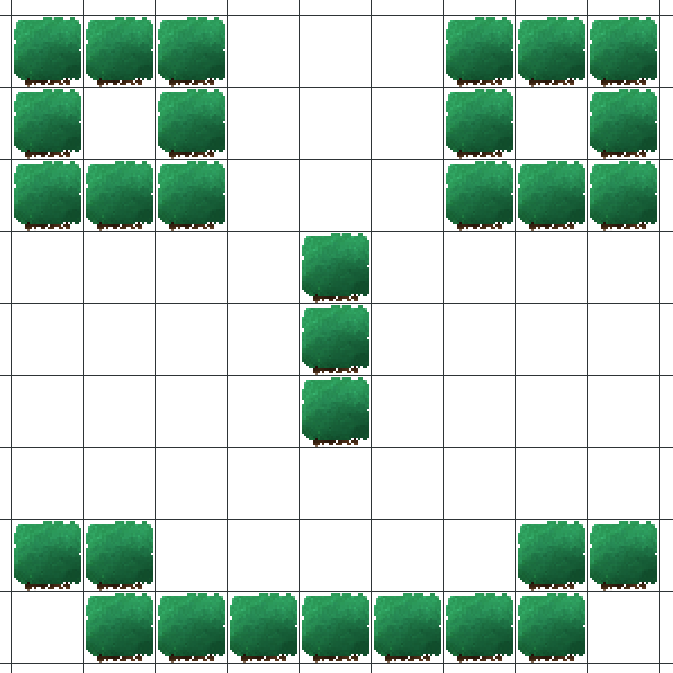
\includegraphics[width=\linewidth]{./figures/smily.png}
    \item Zeichne das Smiley mit hilfe von shapes. Du kannst dafür z.B. die Pixel shape verwenden.
    \item Erstelle eigene shape klasse für Smilies und geb ihr einen Namen.
    \begin{Infobox}[Eclipse Class wizard]
        Wenn du im Package Explorer von Eclipse einen Rechtsklick machst, gibt es die Option new.
        Dammit bekommst ein kleines Menü an die Hand um zum Beispiel eine Klasse zu erstellen.
    \end{Infobox}
    \item Füge das Interface Shape hinzu.
    \begin{lstlisting}[title=Interface Syntax,frame=ltr]
        class <ClassName> implements <InterfaceName>
        {
            /...
    \end{lstlisting}
    \begin{Infobox}[Interface]
        Interfaces werden auch als Verträge bezeichnet.
        Wenn wir das Interface Shape hinzufügen, dann gehen wir einen Vertrag ein, das wir ein Shape bauen.
        Das heißt jeder kann unser shape wie jede andere Shape verwenden.
        Dammit das geht müssen wir aber jede Operation haben, die auch im Interface verwendet wird.
        Das machen wir indem wir die Operation (mit dem gleichen Namen, Parametern und Modifern) bei uns rein schreiben und davor (am besten in eine eigene Zeile) \lstinline{@Override}
    \end{Infobox}    
    \item Implementiere den Konstruktor und baue darin das smiley shape zusammen. So wie du es in c) gemacht hast.
    \item Eine shape muss eine ganz bestimmte Operation von Interface Überschreiben, nämlich \lstinline{public Iterator<Position> iterator()}.
    Darin brauchen wir aber die shape die wir vorhin bereits erstellt haben.
    Die steht aber in einer Variable vom Konstruktor.
    Die lösung ist einfach: Wir ziehen die Variable aus dem Konstruktor, direkt in die Klasse.
    Wie bei den Operationen schreiben wir auch hier einfach mal ein modifier davor. Diesmal aber \lstinline{private}.
    Nun kann jede Operation und Konstruktor dieselbe Variable verwenden.

    Wir wollen jetzt aber nicht einen eigenen Iterator schreiben oder kreieren. Also geben wir einfach zurück, was die iterator funktion der Pixel shape, uns zurückgibt.
    \item Wie eine Operation kann auch ein Konstruktor Parameter haben.
    Erstelle einen oder Mehrere, mit denen du eine Position mit geben kannst, an der das Smiley gezeichnet wird
    und zeichen ein paar an verschiedenen postionen.
\end{enumerate}

\newpage
